\documentclass[12pt]{article}
\usepackage{alltt}
\usepackage[utf8]{inputenc}
\usepackage[dvips]{graphicx}
%\usepackage{a4wide}
\usepackage{epsfig}
\usepackage{fancybox}
\usepackage{verbatim}
\usepackage{array}
\usepackage{latexsym}
\usepackage{alltt}
%\usepackage{dsfont}
\usepackage{caption}
\usepackage{subcaption}
%\usepackage{fullpage}
\usepackage{hyperref}
\usepackage{textcomp}
\usepackage{listings}
\usepackage{color}
\usepackage{amsmath}
\usepackage{amsfonts}
\usepackage{tikz}
\usepackage{float}
\usepackage{matlab-prettifier}
\usepackage{graphicx}



\topmargin=-1.8cm
\addtolength{\textheight}{6.5cm}
\addtolength{\textwidth}{2.0cm}
\setlength{\oddsidemargin}{0.0cm}
\setlength{\evensidemargin}{0.0cm}

\newcommand{\HRule}{\rule{\linewidth}{1mm}}

\usepackage{tikz}
\usetikzlibrary{trees}
\tikzset{
  font={\fontsize{7pt}{12}\selectfont}}
  
\newcommand{\Q}{\raisebox{1.7pt}{$\scriptstyle\bigcirc$}}

\lstset{
    %backgroundcolor=\color{lbcolor},
    tabsize=2,
    language=C++,
    basicstyle=\footnotesize,
    numberstyle=\footnotesize,
    aboveskip={0.0\baselineskip},
    belowskip={0.0\baselineskip},
    columns=fixed,
    showstringspaces=false,
    breaklines=true,
    prebreak=\raisebox{0ex}[0ex][0ex]{\ensuremath{\hookleftarrow}},
    %frame=single,
    showtabs=false,
    showspaces=false,
    showstringspaces=false,
    identifierstyle=\ttfamily,
    keywordstyle=\color[rgb]{0,0,1},
    commentstyle=\color[rgb]{0.133,0.545,0.133},
    stringstyle=\color[rgb]{0.627,0.126,0.941},
}

\usepackage[]{mdframed}
\usepackage{enumitem}

\usepackage{titlesec}
\titleformat{\subsection}[runin]{}{}{}{}[]









\begin{document}

% Set the overall layout of the tree
\tikzstyle{level 1}=[level distance=2.5cm, sibling distance=20em]
\tikzstyle{level 2}=[level distance=2.5cm, sibling distance=10em]

% Define styles for bags and leafs
\tikzstyle{bag} = [text width=16em, text centered, align=center]
\tikzstyle{end} = [circle, minimum width=3pt,fill, inner sep=0pt]

\noindent
\HRule \\[3mm]
\small
\begin{tabular}[b]{lp{4.3cm}r}
Middle East Technical University &  &
Department of Computer Engineering \\
\end{tabular} \\
\begin{center}

                 \LARGE \textbf{CENG 280} \\[4mm]
                 \Large Formal Languages and Abstract Machines \\[4mm]
                \normalsize Spring 2022-2023 \\
                    \Large Homework 3 \\
\end{center}
\HRule



% Write down your name, surname, and student ID below.
\begin{center}
Name Surname:Doruk Berke Yurtsizoglu   \\
Student ID: 2522225
\end{center}



\section*{Answer for Q1}

\subsection*{a.} 
At first, we will create two sections for our states. First one will consists of non-final states, and the other one will only include the final states of our automata.\\
$-$ $G_1$ = $(q_0, q_1, q_3, q_4)$\\
$-$ $G_2$ = $(q_2, q_5)$\\
\\
Now, we will iterate within these groups and inspect their transitions to other states. The rule when iterating is, if you find a different type of transitions  for a state, create a new group for that state and so on. We will stop if we find the same groups from the previous iteration.\\
\\
\begin{table}[H]
        \centering
        \begin{tabular}{|c|c|c|}
		\hline
		State & a & b\\
		\hline
		$q_0$ & $q_1$ & $q_2$\\
		$q_1$ & $q_1$ & $q_2$\\
		$q_2$ & $q_2$ & $q_3$\\
		$q_3$ & $q_4$ & $q_5$\\
		$q_4$ & $q_0$ & $q_2$\\
		$q_5$ & $q_2$ & $q_3$\\
		\hline
               
        \end{tabular}
        

    \end{table}{}

Let's interpret the relation table:\\
$-$ For $q_0$, it goes to a non-final state when reading 'a', and to a final state when reading 'b'.\\ 
$-$ For $q_1$, it goes to a non-final state when reading 'a', and to a final state when reading 'b'.\\
$-$ For $q_2$, it goes to a final state when reading 'a', and to a non-final state when reading 'b'.\\
$-$ For $q_3$, it goes to a non-final state when reading 'a', and to a final state when reading 'b'.\\
$-$ For $q_4$, it goes to a non-final state when reading 'a', and to a final state when reading 'b'.\\
$-$ For $q_5$, it goes to a final state when reading 'a', and to a non-final state when reading 'b'.\\
\\
If we classify our states according to the informations above, we will get:\\
$-$ $C_1$ = $(q_0, q_1, q_3, q_4)$\\
$-$ $C_2$ = $(q_2, q_5)$\\
\\
We can observe that the groups $G_1$-$C_1$ and $G_2$-$C_2$ are identical. This means, we need to stop iterating. We have reach the minimized version of the automata which looks like:\\

\begin{center}
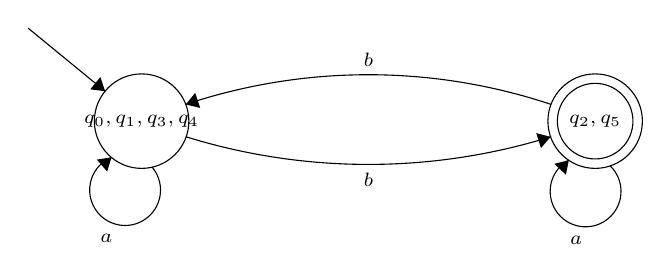
\begin{tikzpicture}[scale=0.2]
\tikzstyle{every node}+=[inner sep=0pt]
\draw [black] (16.5,-21.2) circle (3);
\draw (16.5,-21.2) node {${q_0,q_1,q_3,q_4}$};
\draw [black] (45.3,-21.2) circle (3);
\draw (45.3,-21.2) node {${q_2,q_5}$};
\draw [black] (45.3,-21.2) circle (2.4);
\draw [black] (42.471,-22.197) arc (-72.78508:-107.21492:39.098);
\fill [black] (42.47,-22.2) -- (41.56,-21.96) -- (41.86,-22.91);
\draw (30.9,-24.45) node [below] {$b$};
\draw [black] (19.304,-20.135) arc (108.45084:71.54916:36.64);
\fill [black] (19.3,-20.14) -- (20.22,-20.36) -- (19.9,-19.41);
\draw (30.9,-17.75) node [above] {$b$};
\draw [black] (17.161,-24.114) arc (40.50427:-247.49573:2.25);
\draw (14.27,-28.33) node [below] {$a$};
\fill [black] (14.59,-23.5) -- (13.66,-23.64) -- (14.31,-24.4);
\draw [black] (46.248,-24.034) arc (46.23483:-241.76517:2.25);
\draw (44.09,-28.48) node [below] {$a$};
\fill [black] (43.63,-23.68) -- (42.71,-23.91) -- (43.44,-24.6);
\draw [black] (9.3,-15.3) -- (14.18,-19.3);
\fill [black] (14.18,-19.3) -- (13.88,-18.4) -- (13.24,-19.18);
\end{tikzpicture}
\end{center} 

 
\subsection*{b.}    

There are two equivalence classes for this automata:\\
1-) Strings that have even number of b's\\
2-) Strings that have odd number of b's\\
\\
Let's define these equivalence classes with regular expressions:\\
(e) = ($a^* \cup a^* b a^* b a^* (b a^* b a^* )^* $) = $Lb$\\ 
(b) = ($a^* b a^* (b a^* b a^* )^* $) = $L$\\
Note: $L$ = Strings that have odd number of b's.\\


\subsection*{c.} 
.\\
Let string1 ($s_1$) = $a^n b^m c^k$\\
Let string2 ($s_2$) = $a^x b^y c^z$ where $n \neq x, m \neq y, k \neq z$ .\\
Let string3 ($s_3$) = $d^u$ where u satisfies $m+n = k+2u$ .\\ 
\\
If we concatenate $s_1$ and $s_3$ ($s_1 s_3$) we get strings in the format of   $a^n b^m c^k d^u $ which are in our language $L'$.\\
However if we do the same thing with $s_2$ and $s_3$ ($s_2 s_3$), the new string can't be in $L'$ since $n \neq x, m \neq y, k \neq z$ .\\
\\
Therefore, we can conclude that $\approx_L$ has infinetly many equivalence classes and hence by MyHill-Nerode Theorem $L'$ is not regular.
 

\section*{Answer for Q2}
\subsection*{1.} 

G = (V, $\sum$, R, S) where \\
$\sum$ = (a,b), V = (S, A, X)$\cup$ $\sum$\\
\\
R =\\ 
S $\rightarrow$ Ab $|$ XS $|$ SXA \\
A $\rightarrow$ Ab $|$ e \\
X $\rightarrow$ e $|$ XX $|$ aXb $|$ bXa \\
\\
A variable is equal to $b^*$ which makes the strings of this grammar unbalanced.\\
X variable irepresents the balanced parts of the strings.\\
S determines where the unbalanced part is. It can be at the beginning, in the middle or at the end.\\ 


\subsection*{2.} 

G = (V, $\sum$, R, S) where \\
$\sum$ = (0,1,2), V = (S, A, X)$\cup$ $\sum$\\
\\
R =\\ 
S $\rightarrow$ AX \\
A $\rightarrow$ 0A1 $|$ e \\
X $\rightarrow$ 1X2 $|$ e \\
\\
Separate the desired string ($0^i 1^j 2^k$) into two parts:\\
$-$ $0^i 1^i$\\
$-$ $1^k 2^k$\\
This way, we will have i + k amount of 1's in our strings.\\
\\
A variable is equal to $0^i 1^i$.\\
X variable is equal to $1^k 2^k$.\\
S variable concatenates A and X.\\

\subsection*{3.} 

G = (V, $\sum$, R, S) where \\
$\sum$ = (0,1), V = (S)$\cup$ $\sum$\\
\\
R =\\ 
S $\rightarrow$ 0 $|$ 1 $|$ 0S0 $|$ 0S1 $|$ 1S0 $|$ 1S1 \\
\\
Base cases are  just 0 or 1. We will construct other strings from these base cases.\\
Strings can start with 0 and end with 1, or start with 0 and end with 0, or start with 1 and end with 1, or start with 1 and end with 0.\\

\begin{center}
\begin{tikzpicture}[scale=0.2]
\tikzstyle{every node}+=[inner sep=0pt]

\draw (37.6,-6.7) node {$S$};

\draw (26.1,-15.6) node {$0$};

\draw (37.6,-15.6) node {$S$};

\draw (48.7,-15.6) node {$0$};

\draw (26.1,-26.3) node {$0$};

\draw (37.6,-26.3) node {$S$};

\draw (48.7,-26.3) node {$0$};

\draw (37.6,-37.3) node {$S$};

\draw (25.7,-36.9) node {$1$};

\draw (48.5,-37.3) node {$1$};

\draw (37.6,-48.8) node {$1$};
\draw [black] (35.23,-8.54) -- (28.47,-13.76);
\fill [black] (28.47,-13.76) -- (29.41,-13.67) -- (28.8,-12.88);
\draw [black] (37.6,-9.7) -- (37.6,-12.6);
\fill [black] (37.6,-12.6) -- (38.1,-11.8) -- (37.1,-11.8);
\draw [black] (39.94,-8.58) -- (46.36,-13.72);
\fill [black] (46.36,-13.72) -- (46.05,-12.83) -- (45.42,-13.61);
\draw [black] (37.6,-18.6) -- (37.6,-23.3);
\fill [black] (37.6,-23.3) -- (38.1,-22.5) -- (37.1,-22.5);
\draw [black] (35.4,-17.64) -- (28.3,-24.26);
\fill [black] (28.3,-24.26) -- (29.22,-24.08) -- (28.54,-23.35);
\draw [black] (39.76,-17.68) -- (46.54,-24.22);
\fill [black] (46.54,-24.22) -- (46.31,-23.3) -- (45.62,-24.02);
\draw [black] (35.36,-28.3) -- (27.94,-34.9);
\fill [black] (27.94,-34.9) -- (28.87,-34.75) -- (28.2,-34);
\draw [black] (39.71,-28.43) -- (46.39,-35.17);
\fill [black] (46.39,-35.17) -- (46.18,-34.25) -- (45.47,-34.95);
\draw [black] (37.6,-29.3) -- (37.6,-34.3);
\fill [black] (37.6,-34.3) -- (38.1,-33.5) -- (37.1,-33.5);
\draw [black] (37.6,-40.3) -- (37.6,-45.8);
\fill [black] (37.6,-45.8) -- (38.1,-45) -- (37.1,-45);
\end{tikzpicture}
\end{center}

\section*{Answer for Q3}

\subsection*{1.} 

Strings that start and end with either 1 or 0.


\subsection*{2.} 

Strings that contain at least two 1's.

\end{document}
